\documentclass[12pt,aspectratio=169,xcolor=dvipsnames,hyperref={colorlinks,urlcolor=iiia_orange}]{beamer}
\usetheme[pageofpages=of,% String used between the current page and the
                         % total page count.
          bullet=circle,% Use circles instead of squares for bullets.
          titleline=true,% Show a line below the frame title.
          alternativetitlepage=true,% Use the fancy title page.
          ]{Torino}

\usecolortheme{iiia}

\usepackage{libertine}
\usepackage[scaled=0.8]{FiraMono}

% definitions

\newcommand{\wrt}{\textit{wrt}}

\newcommand{\titleicon}[2]{%
\makebox[\framewidth]{#1\hfill\raisebox{-0.25ex}{\includegraphics[height=5mm]{img/icons/#2}}}%
}

\newcommand{\icon}[1]{%
\mathord{\raisebox{-0.25ex}{\includegraphics[height=2ex]{#1}}}%
}

\newcommand{\inline}[1] {%
\mathord{\raisebox{-0.5ex}{\includegraphics[height=2.5ex]{img/#1}}}%
}

\makeatletter
\newcommand*{\shiftbox}[2]{%
    \settowidth{\@tempdima}{#2}%
    \makebox[\@tempdima]{\hspace*{#1}#2}%
}
\makeatother

% dashed box

\usepackage{environ}

\NewEnviron{dashedbox}{
    \par
    \begin{tikzpicture}
        \node[rectangle,minimum width=0.9\textwidth] (m) {\begin{minipage}{0.85\textwidth}\BODY\end{minipage}};
        \draw[dashed] (m.south west) rectangle (m.north east);
    \end{tikzpicture}
}

% don't use ugly monospace font for URLs

\urlstyle{same}

% contour text

\usepackage[outline]{contour}

% use title field

\usepackage{authoraftertitle}

% euro symbol

\usepackage[official]{eurosym}

% use Font Awesome icons

\usepackage{fontawesome}

% comment

\usepackage{comment}

% tikz

\usepackage{tikz}
\usepackage{varwidth}
\usetikzlibrary{calc,fit,positioning,shapes}
\usetikzlibrary{decorations.pathreplacing,calc}
\usetikzlibrary{arrows,arrows.meta} % Stealth
\usetikzlibrary{overlay-beamer-styles} % alt
\tikzstyle{label_side}=[anchor=west,align=left,xshift=1mm,font=\scriptsize]
\tikzstyle{label_below}=[anchor=north,align=center,yshift=-5mm,font=\small]
\tikzstyle{label_above}=[anchor=base,align=center,yshift=2mm,font=\small]


\title{\raisebox{5mm}{\textbf{Filippo Bistaffa}}}
\author{\raisebox{-5mm}{\Large\textbf{1\textsuperscript{st} Crash Course on Parallelization}}}
\institute{\texttt{\url{https://github.com/filippobistaffa/phd-day-parallelization}}\\(clone with \texttt{{-}{-}recursive})}

\date{14 November 2023}

\begin{document}

\begin{frame}[t,plain,noframenumbering]
    \titlepage
\end{frame}

\def\border{2mm}

\begin{frame}<{1,2}>[label=types]
    \frametitle{\titleicon{Types of Parallelization}{cpu}}
    \begin{figure}
        \begin{tikzpicture}[
            xscale=5,
            only1/.style = {alt=<1>{opacity=1}{opacity=0.2}},
            only123/.style = {alt=<{1,2,3}>{opacity=1}{opacity=0.2}},
            only124/.style = {alt=<{1,2,4}>{opacity=1}{opacity=0.2}},
        ]
            \def\photosize{3.5cm}
            \node[only123,outer sep=\border,circle,draw,minimum size=\photosize,path picture={
                \node at (path picture bounding box.center){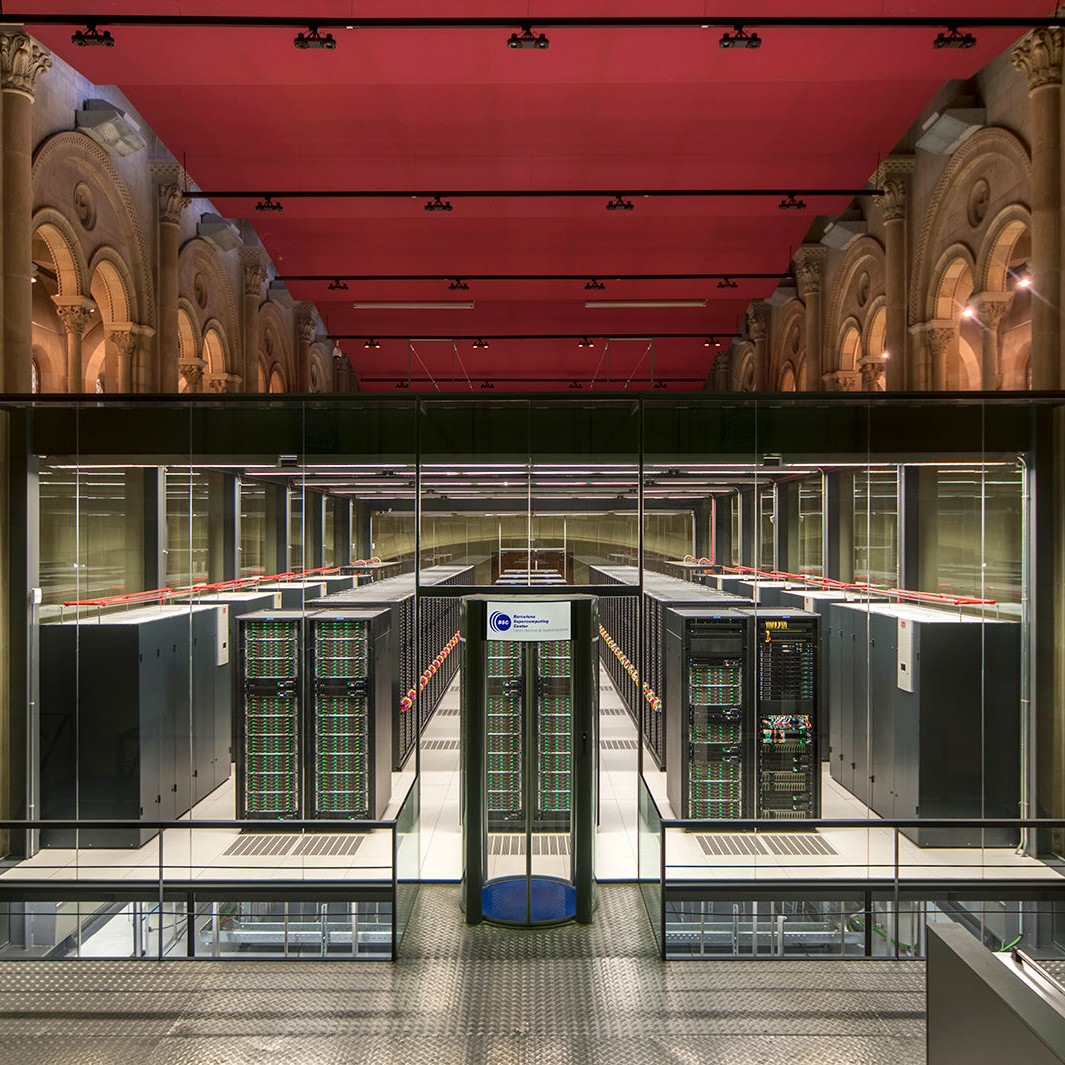
\includegraphics[width=\photosize]{img/marenostrum}};
            }] at (-1.5,0) (cluster) {};
            \node[only123,anchor=north,align=center] at (cluster.south) {Cluster};
            \node[only124,outer sep=\border,circle,draw,minimum size=\photosize,path picture={
                \node at (path picture bounding box.center){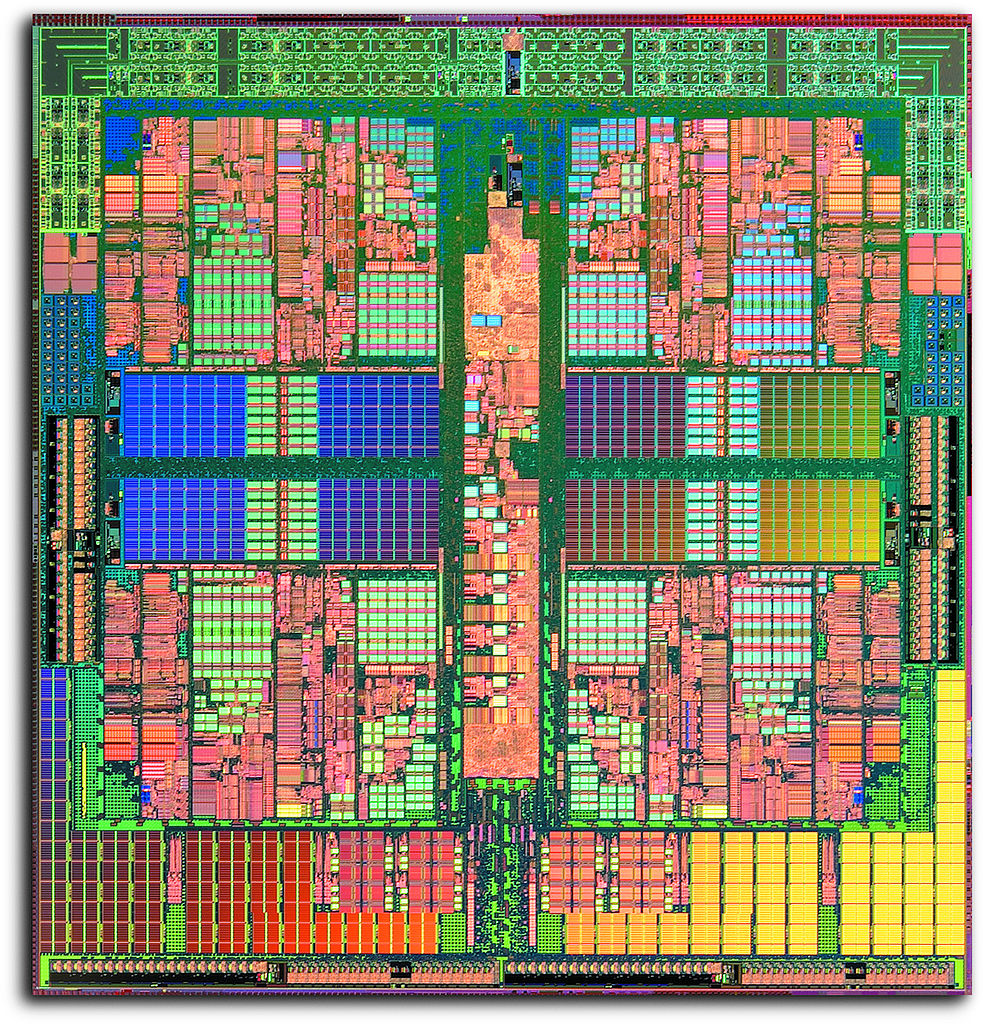
\includegraphics[width=\photosize]{img/multicore}};
            }] at (-0.5,0) (multicore) {};
            \node[only124,anchor=north,align=center] at (multicore.south) {Multi-Core};
            \node[only1,outer sep=\border,circle,draw,minimum size=\photosize,path picture={
                \node at (path picture bounding box.center){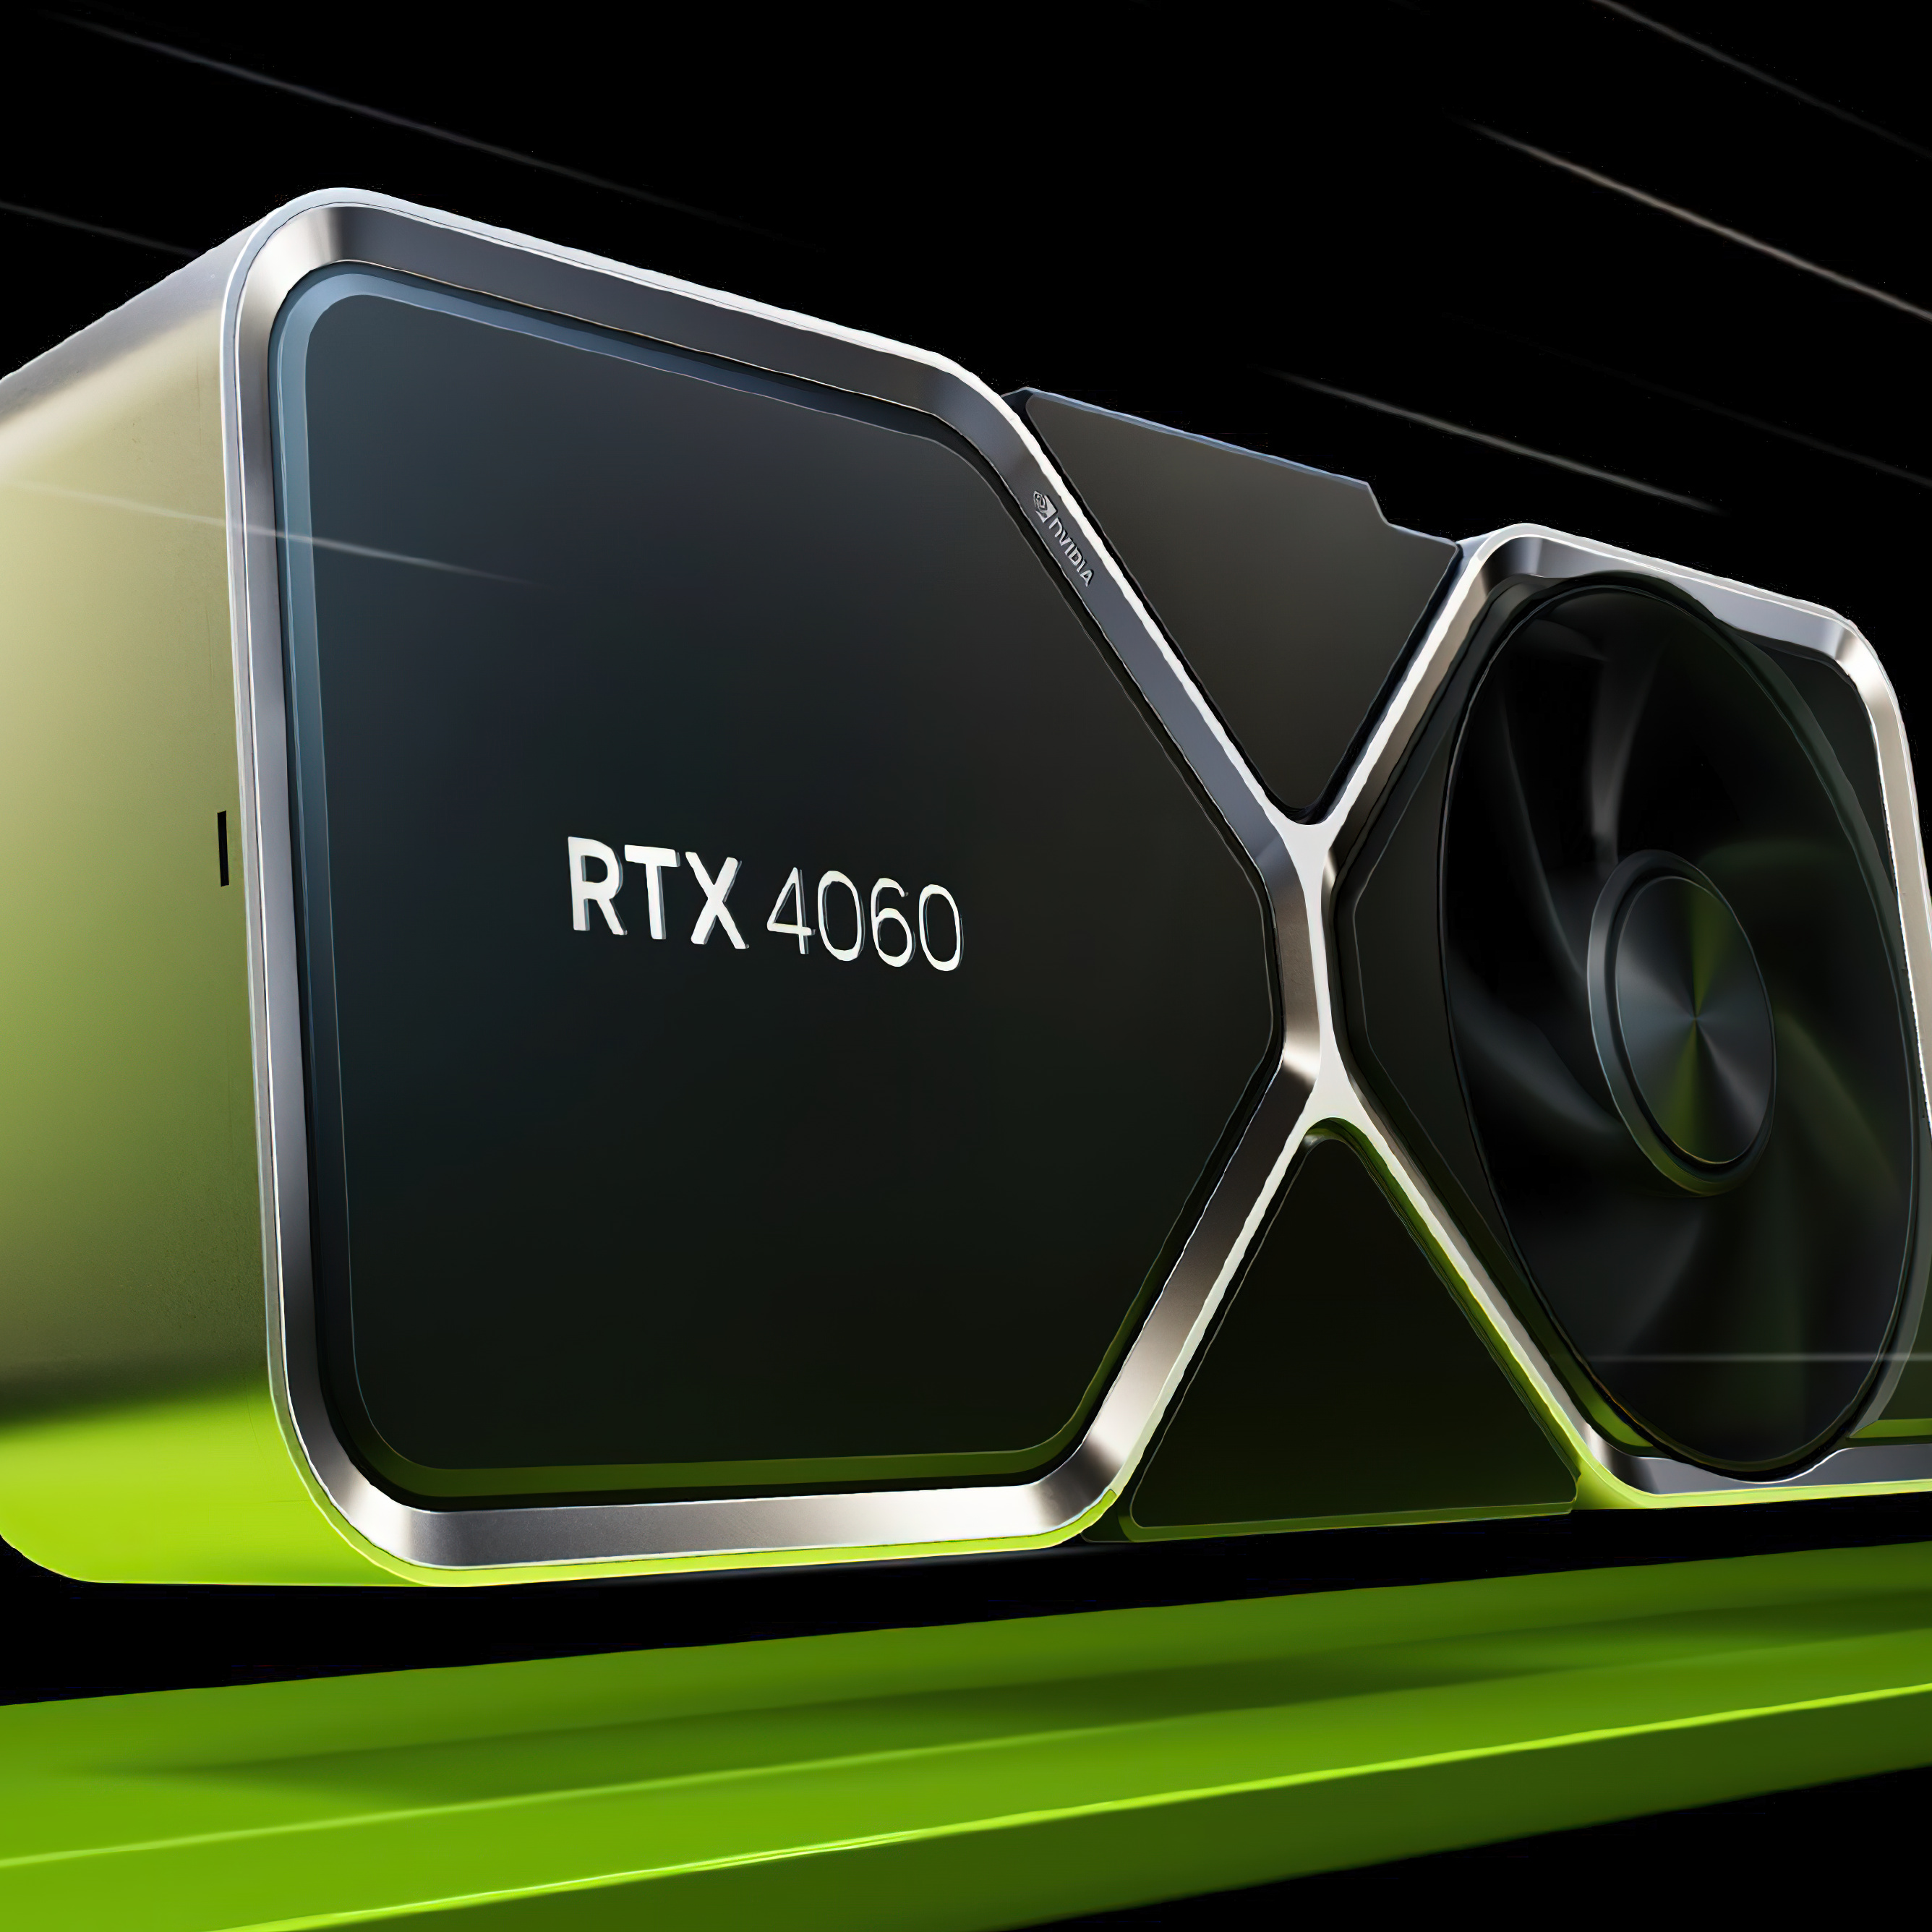
\includegraphics[width=\photosize]{img/nvidia}};
            }] at (0.5,0) (gpu) {};
            \node[only1,anchor=north,align=center] at (gpu.south) {GPU};
        \end{tikzpicture}
    \end{figure}
\end{frame}

\section{Cluster Parallelization}

\againframe<3>{types}

\def\xscale{5.3}

\begin{frame}
    \frametitle<1>{\titleicon{Local Software Execution}{workstation}}
    \frametitle<2>{\titleicon{Cluster Software Execution}{cluster}}
    \begin{figure}
        \begin{tikzpicture}[xscale=\xscale]
            \node at (+1.25,0) {};
            \node at (-1.25,0) {};
            \node[outer sep=\border] at (-1,0) (u) {
\includegraphics[height=2cm]{img/icons/user}};
            \node[anchor=north,align=center] at (u.south) {Programmer};
            \node[outer sep=\border] at (+0,0) (s) {
\includegraphics[height=1cm]{img/icons/software}};
            \node[anchor=north,align=center] at (s|-u.south) {Software};
            \draw[thick,-{Stealth}] (u) -- node[font=\footnotesize,above] {Write\vphantom{Jpy}} node[font=\footnotesize,below] {Software} (s);
            \only<1>{
                \node[outer sep=\border] at (+1,0) (w) {
\includegraphics[height=2cm]{img/icons/workstation}};
                \node[anchor=north,align=center] at (w|-u.south) {Workstation};
                \draw[thick,-{Stealth}] (s) -- node[font=\footnotesize,above] {Execute\vphantom{Jpy}}
                                               node[font=\footnotesize,below] {Software} (w);
            }
            \only<2>{
                \node[outer sep=\border] at (+1,0) (w) {
\includegraphics[height=2cm]{img/icons/cluster}};
                \node[anchor=north,align=center] at (w|-u.south) {\href{https://informatica.doc.iiia.csic.es/cap-ia/}{CAP-IA}};
                \draw[thick,-{Stealth}] (s) -- node[font=\footnotesize,above] {Execute\vphantom{Jpy}} 
                                               node[font=\footnotesize,below] {Software}
                                               node[opacity=0.7] {
\includegraphics[height=15mm]{img/icons/forbidden}} (w);
            }
        \end{tikzpicture}
    \end{figure}
\end{frame}

\begin{frame}{\titleicon{Cluster Software Execution}{cluster}}
    \begin{figure}
        \begin{tikzpicture}[xscale=\xscale]
            \node at (+1.25,0) {};
            \node at (-1.25,0) {};
            \node[outer sep=\border] at (-1,0) (u) {
\includegraphics[height=2cm]{img/icons/user}};
            \node[outer sep=\border] at (+1,0) (c) {
\includegraphics[height=2cm]{img/icons/cluster}};
            \node[outer sep=\border] at ($(u)!0.33333!(c)$) (s) {
\includegraphics[height=1cm]{img/icons/software}};
            \node[outer sep=\border] at ($(u)!0.66666!(c)$) (l) {
\includegraphics[height=2cm]{img/icons/server_network}};
            \draw[thick,-{Stealth}] (u) -- node[font=\footnotesize,above] {Write\vphantom{Jpy}} node[font=\footnotesize,below] {Software} (s);
            \draw[thick,-{Stealth}] (s) -- node[font=\footnotesize,above] {Copy\vphantom{Jpy}} node[font=\footnotesize,below] {Software} (l);
            \draw[thick,-{Stealth}] (l) -- node[font=\footnotesize,above] {Submit\vphantom{Jpy}} node[font=\footnotesize,below] {Job} (c);
            \node[anchor=north,align=center] at (u.south) {Programmer};
            \node[anchor=north,align=center] at (s|-u.south) {Software};
            \node[anchor=north,align=center] at (l|-u.south) {\texttt{vega.iiia.csic.es}};
            \node[anchor=north,align=center] at (c|-u.south) {\href{https://informatica.doc.iiia.csic.es/cap-ia/}{CAP-IA}};
        \end{tikzpicture}
    \end{figure}
\end{frame}

\newcommand{\giturl}[1]{\href{https://github.com/filippobistaffa/phd-day-parallelization/blob/main/#1}{\texttt{#1}}}

\begin{frame}{\titleicon{Today's Menu}{list}}
    \begin{itemize}
        \setlength\itemsep{-1pt}
        \item[\faGithub] Python hello world!
        \item[] \giturl{cluster-parallel/hello.sh}
        \item[\faGithub] Compile \href{https://github.com/ggerganov/llama.cpp}{\texttt{llama.cpp}}, a C++ LLM framework
        \item[] \giturl{cluster-parallel/compile-llama.sh}
        \item[\faGithub] Download the \href{https://lmsys.org/blog/2023-03-30-vicuna}{``Vicuna-13B''} LLM for \texttt{llama.cpp} on \texttt{beegfs}
        \item[] \giturl{cluster-parallel/download-model-beegfs.sh}
        \item[\faGithub] Generate a course description with \texttt{llama.cpp}
        \item[] \giturl{cluster-parallel/description.sh}
        \item[\faGithub] Compile \texttt{llama.cpp} with GPU support
        \item[] \giturl{cluster-parallel/compile-llama-gpu.sh}
        \item[\faGithub] Generate a course description with \texttt{llama.cpp} with GPU support
        \item[] \giturl{cluster-parallel/description-gpu.sh}
    \end{itemize}
\end{frame}

\section{Multi-Core Parallelization}

\againframe<4>{types}

\begin{frame}{\titleicon{Today's Menu}{list}}
    \begin{itemize}
        \setlength\itemsep{-1pt}
        \item[\faGithub] Setup CMake to compile C++ examples
        \item[] \giturl{cpu-parallel/CMakeLists.txt}
        \item[\faGithub] Basic sequential \texttt{for} loop
        \item[] \giturl{cpu-parallel/basic-loop.cpp}
        \item[\faGithub] Basic parallel \texttt{for} loop with \href{https://www.openmp.org}{OpenMP}
        \item[] \giturl{cpu-parallel/basic-loop-openmp.cpp}
        \item[\faGithub] Static \textit{vs} dynamic scheduling
        \item[] \giturl{cpu-parallel/dynamic-scheduling.cpp}
        \item[\faGithub] Parallel sum-reduction with \texttt{reduction}
        \item[] \giturl{cpu-parallel/parallel-reduction.cpp}
        \item[\faGithub] Parallelized \textit{vs} un-parallelized sections (\href{https://en.wikipedia.org/wiki/Amdahl\%27s_law}{Amdahl's law})
        \item[] \giturl{cpu-parallel/amdahl-law.cpp}
    \end{itemize}
\end{frame}

\end{document}
